%
%   Data Analysis
%       - ANOVA and Regression and stuff.
%   
\section{Inferential statistics}
\label{section:infer_stats}

As stated in our Report's title, the main focus of the analysis will be \textit{Thermal Design Power} and the affect of
other attributes (variables) on this dependent variable.

\textit{Thermal Design Power} \verb|TDP| is an interesting characteristic that comes with the CPU. Theoretically, this is the
maximum amount of heat that can be released by its cooling system, which should never be exceeded. This characteristic somehow
represents the heat barrier of a processor, and if its cooling system is designed to deal with almost all the heat it release,
\verb|TDP| roughly equates to its power consumption. The higher the \verb|TDP|, the better the CPU's cooling system, but also 
demonstrates the amount of energy consumption required to dissipate the heat.

The reason why we did not use \textit{Temperature} but instead \textit{Thermal Design Power} is that we want to find the amount of
energy needed to keep the CPU operational properly, not the temperature point that the CPU can work but be potentially damaged.

We would try to utilize some Regression models to predict its \verb|TDP| via other configurations (or determinants) such as
\textit{Thermal design power}, \textit{Number of cores}, \textit{Base frequency}, \textit{Temperature}, \textit{Lithography} and its \textit{Status}.
%\textit{Market} and its \textit{Status}.% Also, we will see if with the determined \verb|TDP|, we can classify the CPU, whether
%it belongs to mass computing devices (Server) or personal usage (Desktop and Mobile).



\subsection{Data preparation}

First, we load the cleaned data set from the cleaning process above.

\begin{code}{R}
pacman::p_load(
    rio,     # for imports & exports
    ggplot2, # for plots
    zoo,      # for year-quarter formats
    car     # for levent and shapiro
)
data <- import("cpu-clean.csv") # rio::import
\end{code} 

Refer to \textbf{[Figure 7]} and our statement previously, the occurrences of values $\ge 150$ is rare, we decided to
cut them out from our data set.
\begin{code}{R}
    data <- data[data$tdp < 150, ]
\end{code} 

Because we would make use of Regression models to capture the relationships, a Test Set and a Training Set must be present to perform 
cross-validation to test the fitness of the model, besides visualization method by drawing graphs and checking other coefficients. The original
data set is splitted into two smaller sets, training set and validated set (or test set). In detail, 80% data is used for training set while 20% 
is used for test set.

\begin{code}{R}
set.seed(123)

train_indices <- sample(1:nrow(data), nrow(data) * 0.8)
train <- data[train_indices, ]
test <- data[-train_indices, ]
\end{code}

\begin{itemize}
    \item To make a random generation homogeneous among all our tests, we specified a seed (123). Each time we run the cell, we would get
    consistent results of the split.
    \item \verb|sample()| helps us to take a sample from all the elements of our data set using without replacement. The return value of this function
    are the indices of 80% the data set, randomly chosen.
    \item After that, we use a simple indexing technique to assign to a training set and test set, accordingly.
\end{itemize}









\subsection{The relationships between TDP and other factors}
\subsubsection{Hypothesis testing}
\label{section:data_analysis_anova}

To explain further the statements we made above, we will assess the following assumptions by using several techniques such as 
hypothesis testing, ANOVA and computing the covariances.

The assumptions we are aiming to:
\begin{enumerate}
    \item Lithography as a CPU era.
    \item Thermal Design Power with respect to lithography.
    % \item Thermal Design Power with respect to Temperature.
\end{enumerate}



\subsubsection{Lithography as a CPU era.\label{Litho era}}

In this small section, we will demonstrate why \textbf{Lithography as a better representative than Launch date}. To do that, we start by looking at the confidence interval and the visualizations of Lithography over the years.

\begin{code}{R}
    data$litho <- as.factor(data$litho)
    retval <- data.frame(NA, NA, NA, NA)
    names(retval)<-c("5% quantile","95% quantile", "STD Mean", "Confidence Interval")
    for (lit in levels(data$litho))
    {
          quants <- quantile(
            data[data$litho == lit, ]$ldate,
            na.rm = T,
            probs = c(0.05,0.95)
          )
          dates <- data[data$litho == lit, ]$ldate
          new_row <- data.frame(quants[1], quants[2], mean(sd(dates, na.rm=TRUE), na.rm=TRUE),quants[2]-quants[1])
          names(new_row)<-c("5% quantile","95% quantile", "STD Mean", "Confidence Interval")
          retval <- rbind(retval, new_row)
          rm(dates)
    }
    rownames(retval) <- c("NULL", levels(data$litho))
    retval <- retval[-1,]
    print(retval)
\end{code}
\begin{figure}[H]
    \centering
    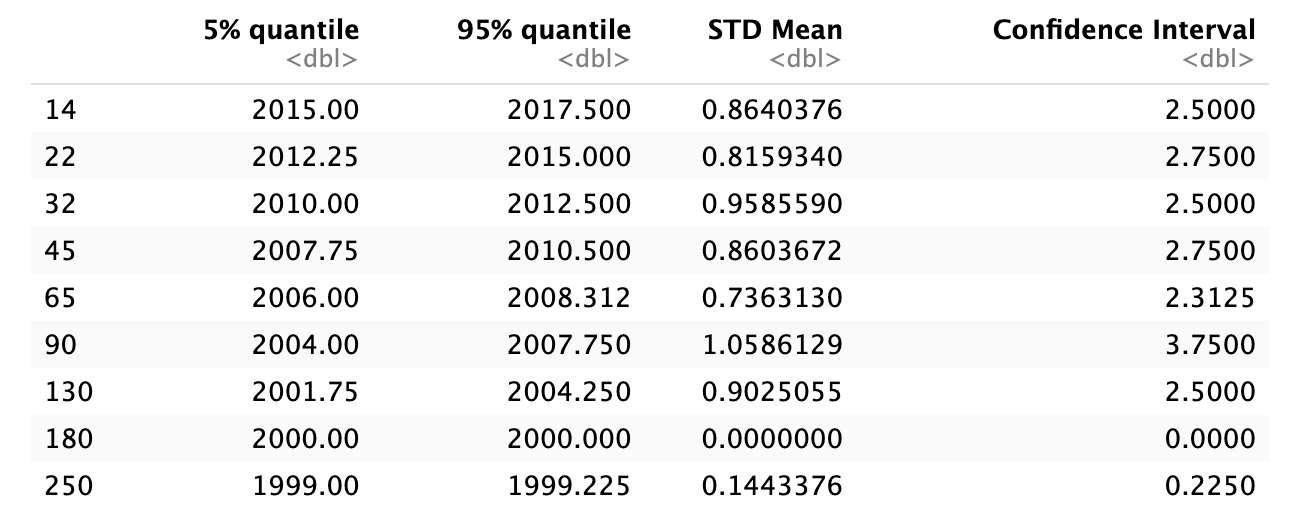
\includegraphics[width=0.5\textwidth]{./graphics/confint_litho.png}
    \caption{Summary of Confidence Interval of Lithography over the years}
\end{figure}

Looking at the Mean of Standard Deviation (\verb|STD Mean|), these \textit{means are pretty stable}, and the \verb|Confidence Interval| column tells us that
most of the era of CPU design \textit{spans for about two and a half years}, and these era are approximately mutually exclusive. This is its big advantage over
using Launch date only, because we can now consider a range of values and group different launch dates together wich possibly share the same characteristics. So,
everytime we wants to refer to a period of CPU, we always use Lithography.





\subsubsection{Thermal Design Power with respect to lithography.}







One more thing we want to emphasize is the \textbf{stability of TDP in recent eras}, and the fact that it is converging. We will do the ANOVA to test and see if there is a significant difference in the tdp between the lithography era.

We will have the null hypothesis:
$H_0$: the mean of the tdp in each type of lithography is the same.
$H_1$: there exists a pair of lithography type so that their mean is different.

From the Descriptive statistics, we can see that there are particularly few CPUs with lithography of 28 and 250, so we will remove them as well as all the row that has \mintinline{R}{NA} value
\begin{code}{R}
    # remove data with few count group ldate and remove NA
    data <- data[data$litho !=28,] 
    data <- data[data$litho !=250,] 

    data <- data[!is.na(data$tdp), ]
    data <- data[!is.na(data$litho), ]
\end{code}

We will create an ANOVA model.

\begin{code}{R}
    litho_anova_model<- aov(tdp ~ litho ,data = data)
\end{code}

Getting the result of the model.

\begin{code}{R}
    summary(litho_anova_model)
\end{code}

\begin{figure}[htbp]
    \centering
    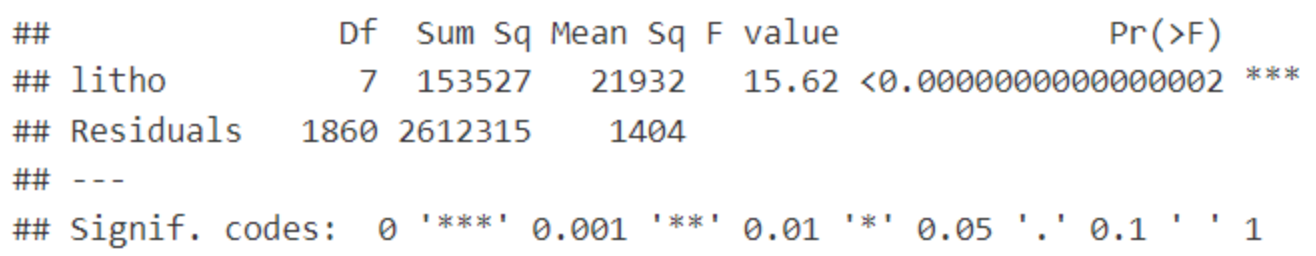
\includegraphics[width = 0.6\textwidth]{graphics/litho_anova_model.png}
\end{figure}

We can see that as the p-value < 0.05, we can reject the null hypothesis $H_0$ and accept the 
alternative hypothesis $H_1$ that there exists a pair of \verb|litho| type so that their \verb|TDP| mean is difference.

To satisfy the requirements of One-way ANOVA, we should check its assumptions on Normality and Homoscedasticity (homogeneous variance).

\begin{code}{R}
    qqPlot(residuals(litho_anova_model))
    shapiro.test(residuals(litho_anova_model))
    leveneTest(tdp ~ litho ,data = data)
\end{code}
\begin{itemize}
    \item We make a Q-Q Plot to explore its residuals.

    \item We perform a Shapiro-Wilk test of Normality:
    
        \qquad Null hypothesis $H_0$ : The residuals of the ANOVA model are normally distributed.

        \qquad Alternative hypothesis $H_1$ : The residuals of the ANOVA model is not normally distributed.

    \item We perform Levene's test to test for the equality of variances.
    
        \qquad Null hypothesis $H_0$ : The variance of \verb|TDP| between categorical \verb|litho| is equal.

        \qquad Alternative hypothesis $H_1$ : The variance between them is not equal.
\end{itemize}

\begin{figure}[H]
    \centering
    \begin{subfigure}[b]{0.35\textwidth}
        \centering
        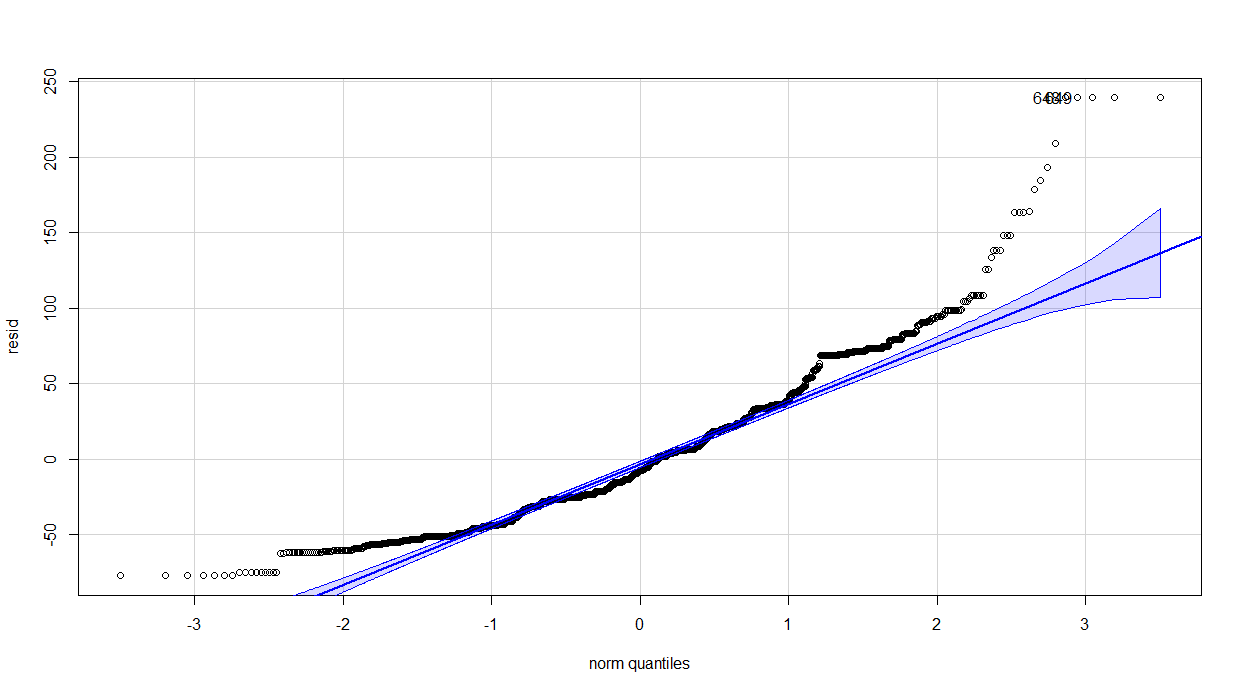
\includegraphics[width=\textwidth]{./graphics/QQplot_resid_litho.png}
        \caption{Q-Q Plot of the ANOVA model}
        \label{fig:anova_litho_shapiro_wilk}
    \end{subfigure}
    \begin{subfigure}[b]{0.6\textwidth}
        \centering
        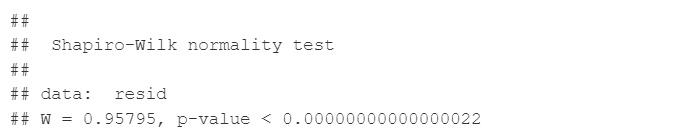
\includegraphics[width=\textwidth]{graphics/shapiro.png}
        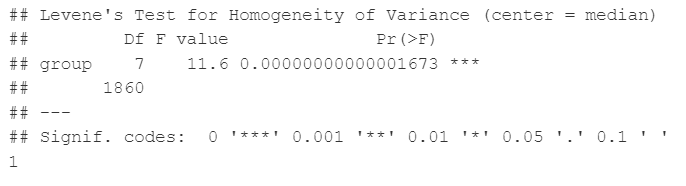
\includegraphics[width=\textwidth]{graphics/levent.png}
        \caption{Results of Shapiro-Wilk and Levene's Test}
        \label{fig:anova_litho_shapiro_wilk}
    \end{subfigure}
    \caption{Summary of the tests.}
\end{figure}

We can see that the normality and variance test both fail as their p-value is both less than 0.05 and the qqplot has a lot of point that deviate from the line, however, the ANOVA test are also resilient against the violation of the two assumptions\cite{tukey}. 

Finally we will analyse the result with a post hoc test to see which mean are different from each other. For this, we will use the TUKEY HSD test for ANOVA.

\begin{code}{R}
    Tukey <- TukeyHSD(litho_anova_model)
    plot(Tukey,las = 2)
\end{code}
\newpage

\begin{figure}[htbp]
    \centering
    % \begin{subfigure}[b]{0.47\textwidth}
    %     \centering
    %     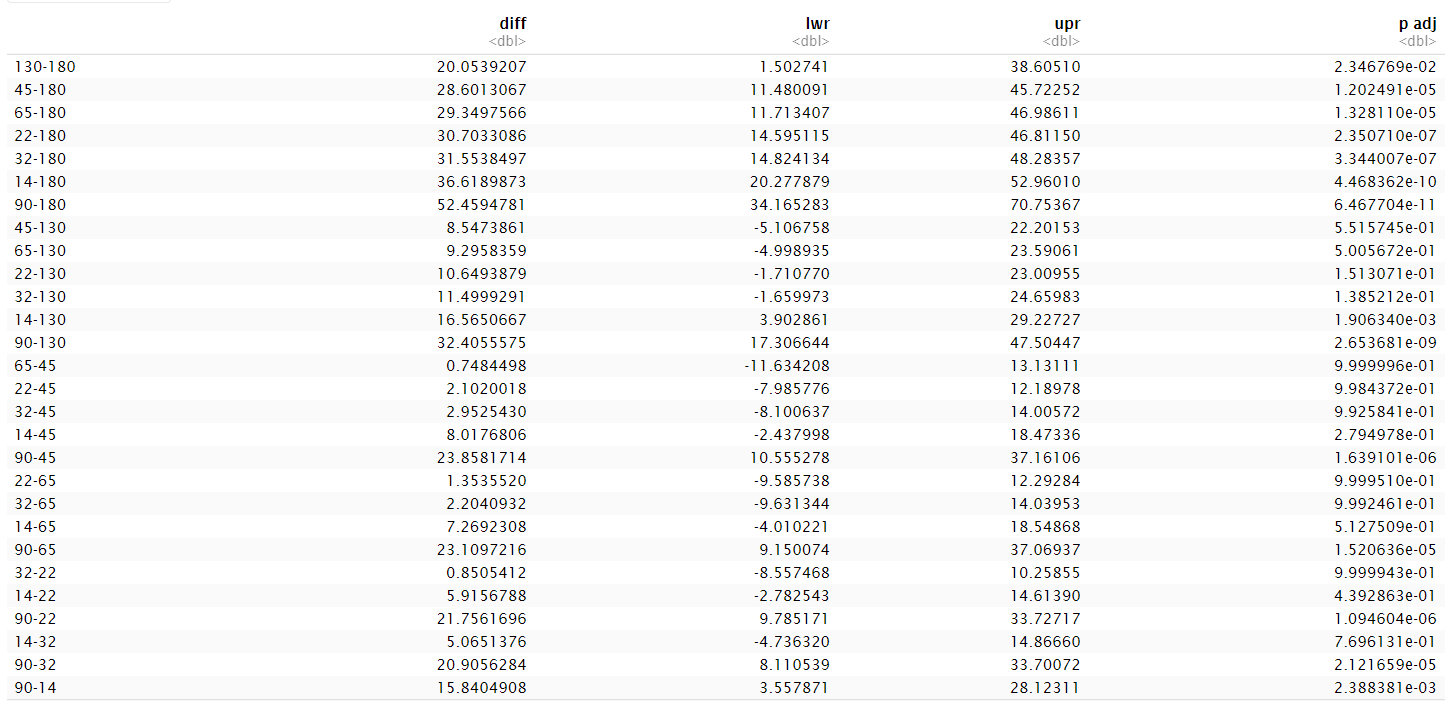
\includegraphics[width=\textwidth]{./graphics/TUKEY HSD.png}
    %     \caption{TUKEY HSD test result}
    %     \label{fig:TUKEY}
    % \end{subfigure}
    % \hfill

    \begin{subfigure}[b]{0.45\textwidth}
        \centering
        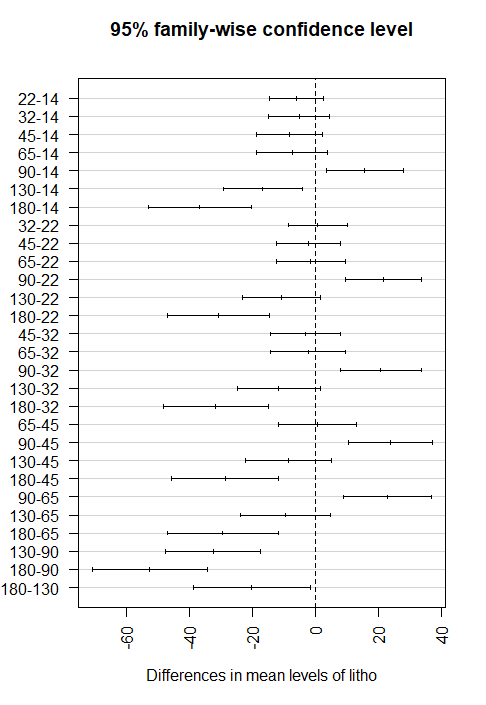
\includegraphics[width=\textwidth]{./graphics/TUKEY HSD confidence.png}
        \caption{TUKEY result plot}
        \label{fig:TUKEYconfidence}
    \end{subfigure}
    \caption{Summary of the post hoc tests.}
\end{figure}
% \begin{figure}
%     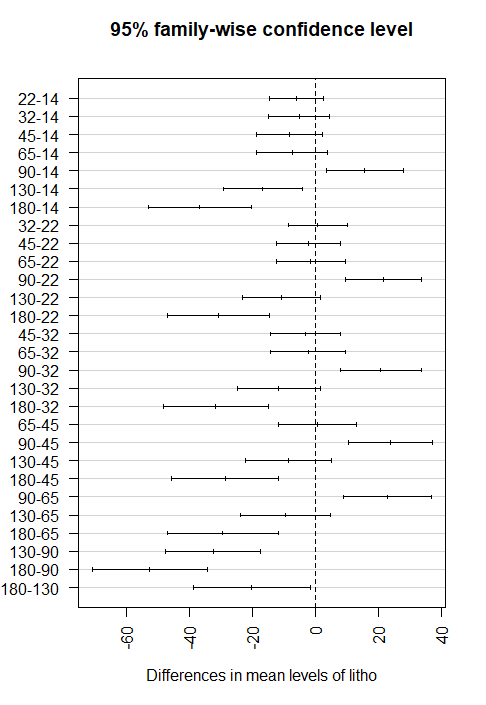
\includegraphics[width= 0.5\textwidth]{./graphics/TUKEY HSD confidence.png}
% \end{figure}
    

% \begin{figure}
%     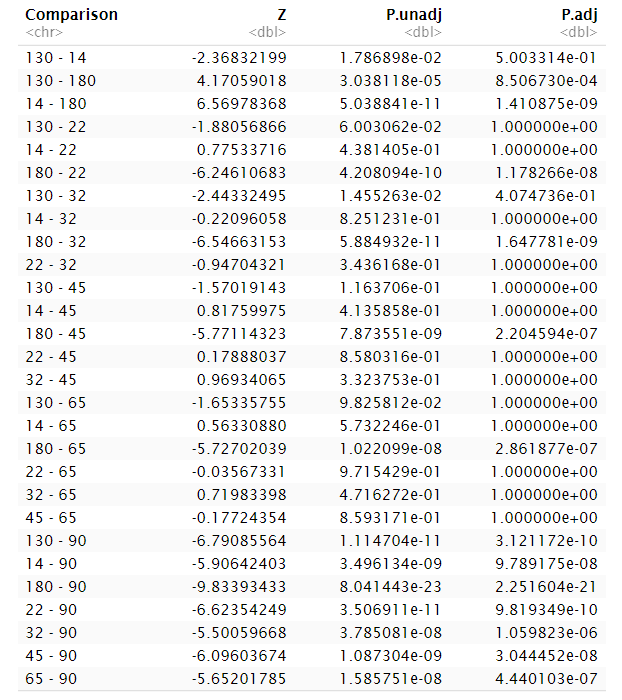
\includegraphics[width= 0.5\textwidth]{./graphics/dunntest.png}
% \end{figure}
We can interpret the result of our data as follow:
\begin{enumerate}
    \item There are a significant difference in \verb|tdp| 's mean and median between the CPU of bigger \verb|lithography|(180,130,90) and CPU of smaller \verb|lithography|(14,22,32,45,65)
    \item The CPU's \verb|lithography| from 14,22,32,45,65 have their mean being relatively the same.
    \item As \verb|lithography| also reflect \verb|release date|, as proven in \ref{Litho era} it also reflect the change in \verb|tdp| of CPU 's design over time.

    
\end{enumerate}

% The trend is clearly show that there are a significant difference in \verb|tdp| between cpu with bigger \verb|lithography|(180,130,90) and cpu of smaller \verb|lithography|(14,22,32,45,65). As have been proven in the  \ref{Litho era} i, we can see that the result also reflect the change in tdp over the year.




% \textbf{Thermal Design Power with respect to Temperature}

% Too really believe there are two trends of \verb|TDP| going on within \verb|temp|, we may want to split the \verb|temp| into
% two halves, one for \verb|temp < 85|, and one for \verb|temp >= 85|. Then we will compute the covariance too see if they are really
% different.

% \begin{itemize}
%     \item If the covariance is positive, the trend is likely to go upward,
%     \item If the covariance is negative, the trend is likely to go downward.
% \end{itemize}

% \begin{code}{R}
%     group1 <- data[data$temp < 85, ]
%     group2 <- data[data$temp >= 85, ]

%     cov(group1$tdp, group1$temp)
%     cov(group2$tdp, group2$temp)
% \end{code}

% The results are as follows:
% \begin{figure}[H]
%     \centering
%     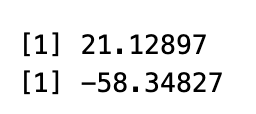
\includegraphics[width=0.3\textwidth]{./graphics/anova_temp_cov.png}
%     \caption{Q-Q plot of Temprature model}
%     \label{fig:anova_temp_cov}
% \end{figure}

% Two covariances are different from each other, meaning that there are two different trends going on.










\subsection{Regression analysis}
\noindent 

Base on checking the linearity of each column related to each other, in this section, we will conduct an investigation on the relationship between thermal design power with other features. There are many types of regression models, including simple linear regression, multiple linear regression, polynomial regression, logistic regression, and more. In this report, we will use certain model to test if there is any significant relationship between these figures.
\subsubsection{Predicting Multi-Linear Model}
\label{section:data_analysis_linear}

Since the scatter plot of the feature \textbf{thermal design power} (tdp) with other variable maybe related to Linear regression.
Now, first of all, we will build a linear regression model using \verb|lm()|.
\begin{code}{R}
# Build the model
model.lr <- lm(tdp ~ ncore + bfreq + temp, data = train)
# Summary of the model
summary(model.lr)
\end{code}

The \verb|summary()| command gives us an overview over some statistics of our model.
\begin{figure}[H]
    \centering
    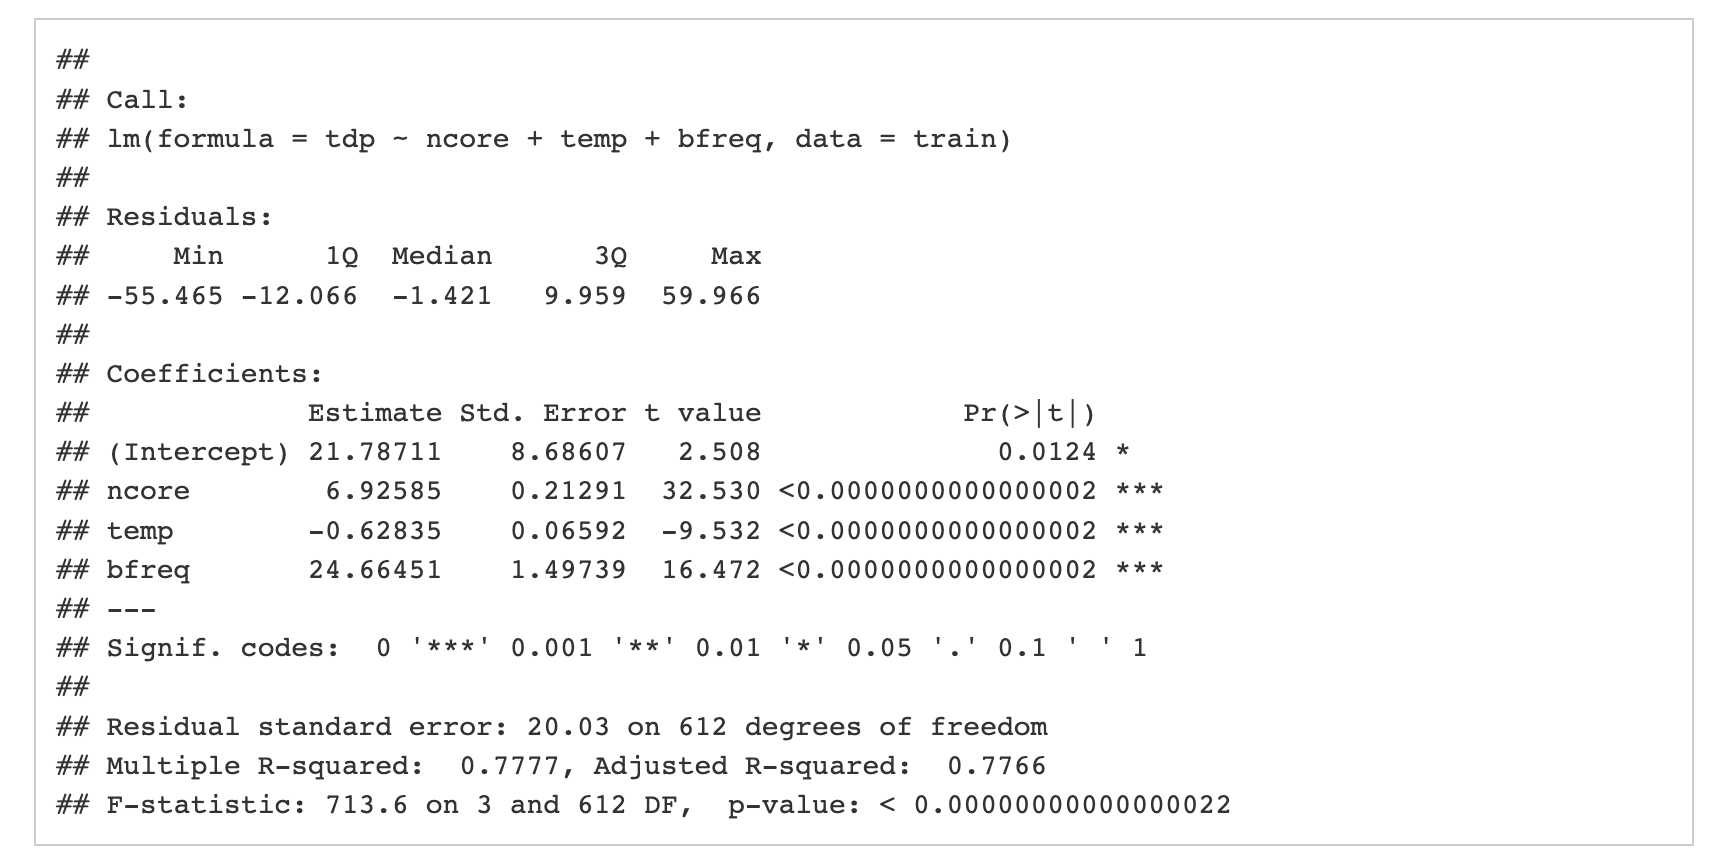
\includegraphics[width=0.8\textwidth]{graphics/linear_summary.png}
    \caption{Summary of linear model}
    \label{fig:30}
\end{figure}
We can observe that all of the variables have the p-value less than 0.05, therefore; all predictors that we have chosen is involved in the building process.

Now we must check for Multiple-Linear model assumption:
\begin{itemize}
    \item Residual Errors have a Mean Value of Zero.
    \item Residual Errors have Constant Variance.
    \item The errors are normally distributed.
\end{itemize}

\textbf{Testing for Residual Errors have a Mean Value of Zero:} We can check this assumption using the histogram of the residual:
\begin{code}{R}
ggplot(model.lr, aes(x = resid(model.lr))) +
  geom_histogram(binwidth = 2, fill = "deepskyblue") # histogram of residuals
\end{code}
\begin{figure}[H]
    \centering
    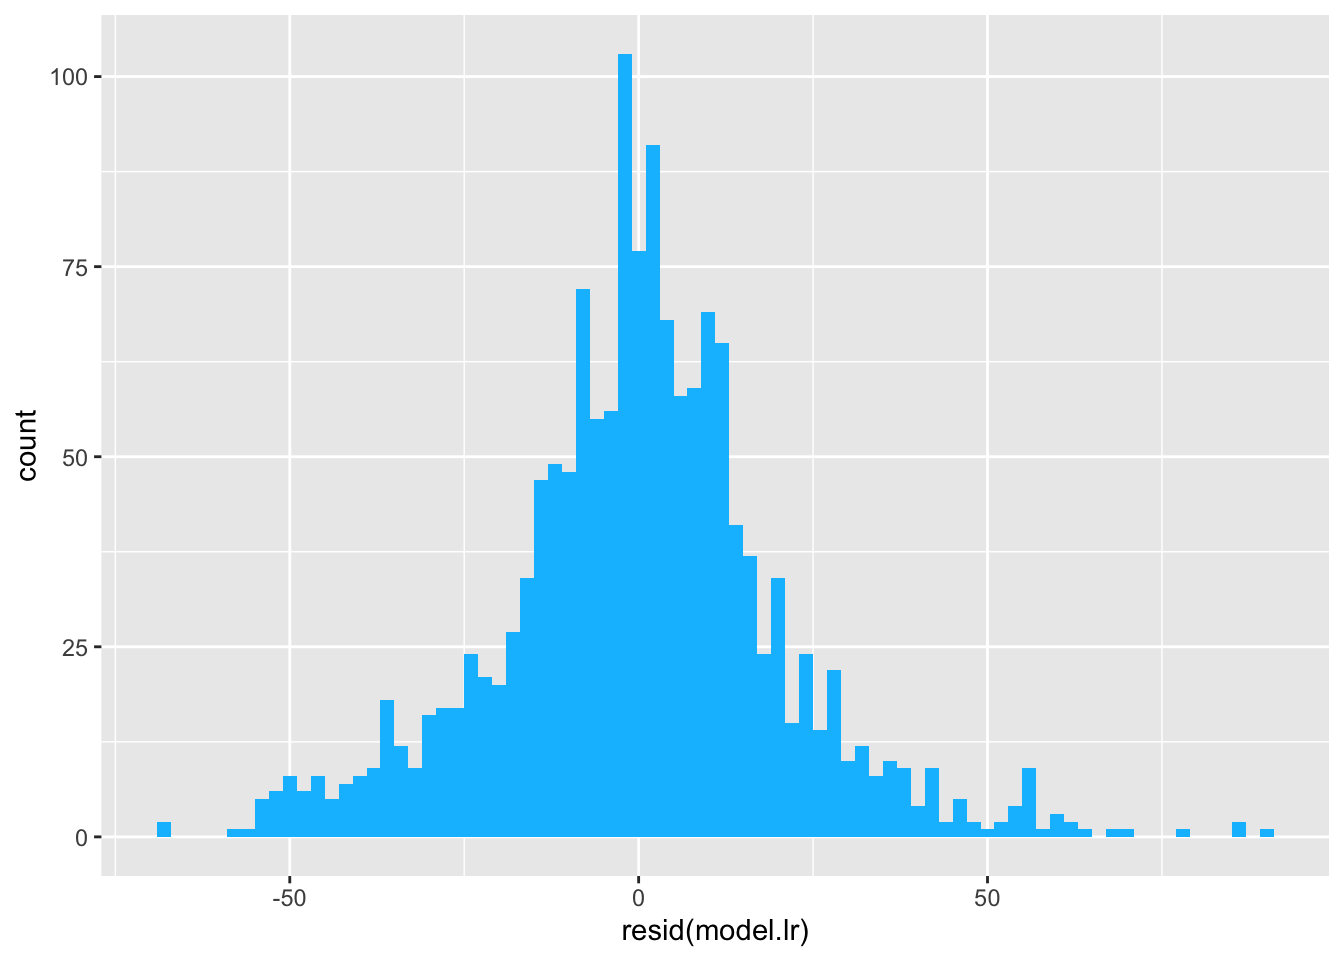
\includegraphics[width=0.8\textwidth]{graphics/linear_mean.png}
    \caption{Histogram of residuals}
    \label{fig:31}
\end{figure}

We can observe that Residuals distribute mainly around the value 0, which is highly indicates that the residuals is scatter mostly around 0 and disperse equally two side of the graph, leading to the fact that the mean is approximately 0. Therefore, this assumption is met.

\textbf{Testing for Residual Errors have Constant Variance:} We can check this assumption using the Scale-Location plot. In this plot we can see the fitted values vs the square root of the standardized residuals. Ideally, we would want to see the residual points equally spread around the red line, which would indicate constant variance.
\begin{code}{R}
plot(model.lr, which = 3)
\end{code}
\begin{figure}[H]
    \centering
    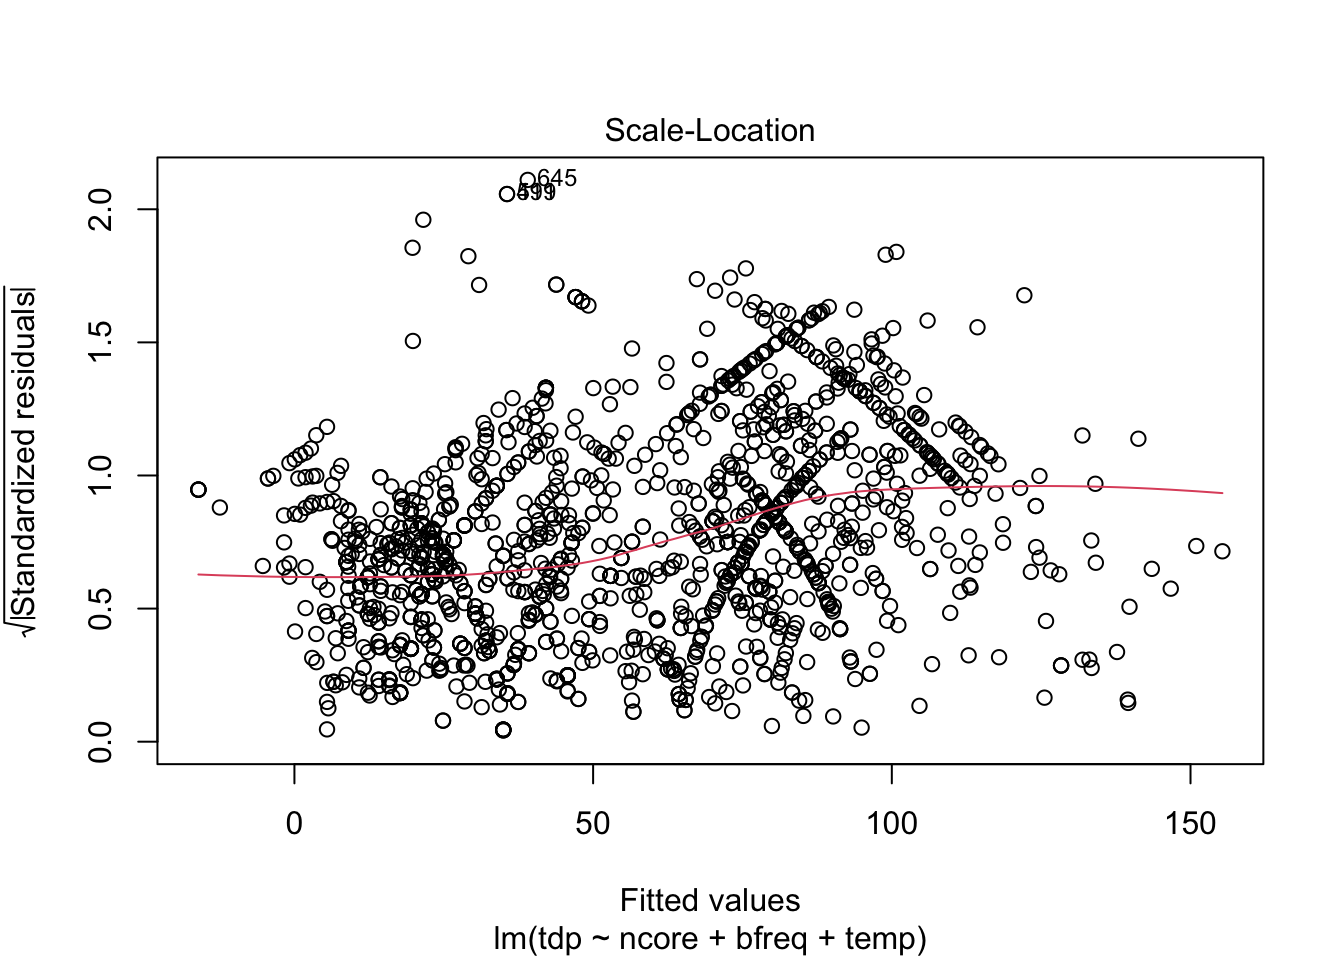
\includegraphics[width=0.8\textwidth]{graphics/linear_scatter.png}
    \caption{Scale-Location plot}
    \label{fig:32}
\end{figure}

In the above plot, we can see that the residual points are equally spread out in a weird pattern, or in other words the residuals scatter is not following any formal distribution and is random. Thus, this assumption is met.

\textbf{Testing for normality of the the errors:} To check this, we have to use Q-Q plot for normality consideration. The output we expect that the residuals will mostly scatter close to the straight line to get normality hypothesis accepted.
\begin{code}{R}
plot(model.lr, which = 2)
\end{code}
\begin{figure}[H]
    \centering
    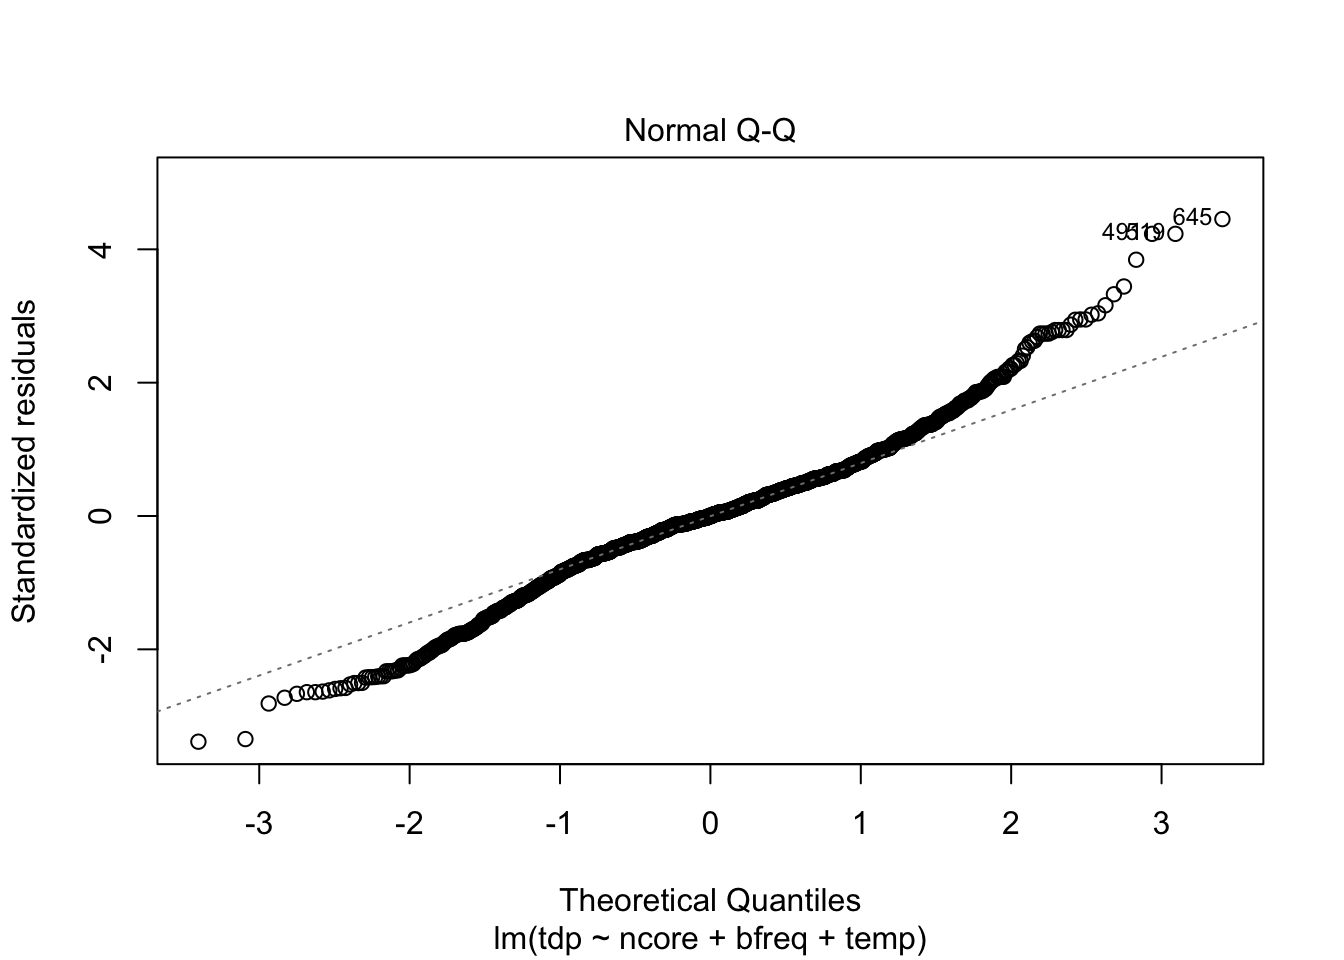
\includegraphics[width=0.8\textwidth]{graphics/linear_normal.png}
    \caption{Q-Q plot for residuals}
    \label{fig:33}
\end{figure}

In the Q-Q plot, it can be seen that those points are lying near the line, while only a few tail points are not lying near the line. We can conclude that this model can be normally accurate, not $100\%$ accurate. Perhaps another model will be more fitted for this data.

When we look at the summary table, the value of multiple $R^2$ is approximately 0.7777, it means that 77.77\% of thermal design power variable is explained by the model and the rest 22.23\% is defined by other factors, which is still accountable but not high. This model so far performing very well.

We will do the scatter plotting for the predicted value of test set compared with real values of the dataset using \verb|plot()| function for more clear vision of this trend.
\begin{code}{R}
# Create data frame for real tdp value and predicted tdp value (for Testing the test set)
comtab.lr <- test['tdp']
comtab.lr['tdp_predicted'] <- as.data.frame(predict(model.lr, newdata = test))
# Plotting
# The majority of points lie near the line, so its ok.
ggplot(comtab.lr, aes(x = tdp, y = tdp_predicted)) +
  geom_point(shape=1, color="blue") +
  geom_abline(mapping=aes(intercept= 0, slope = 1), color="darkblue") +
  labs(x = "TDP", y = "TDP Predicted")
\end{code}
\begin{figure}[H]
    \centering
    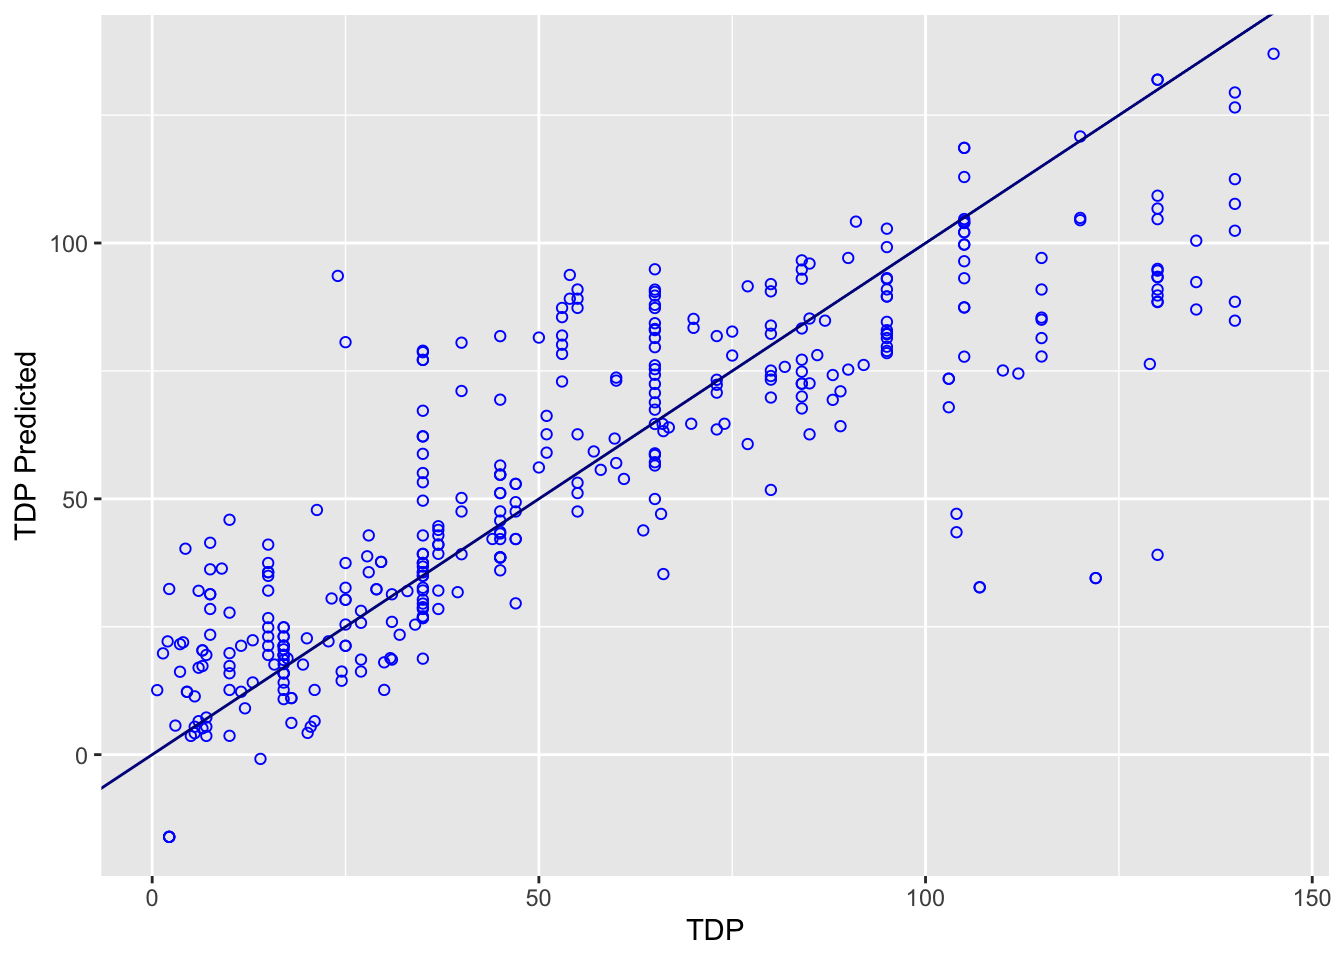
\includegraphics[width=0.8\textwidth]{graphics/linear_predict.png}
    \caption{Predict comparing}
    \label{fig:34}
\end{figure}

At the end of this model, we will do the scatter plotting for the predicted value compared with the real value in test set. The plotted line in graph is $(d): y = x$. The more concentration on this line the more correct the model does.

\textbf{In conclusion}, this model is an acceptable evaluation with the data set, which is shown by the above figures. Nevertheless, the initial assumption about data set's linearity is our subjective point of view, and that is the reason why we continue with the next model.


\subsubsection{Random Forrest Regression Model}
\label{section:data_analysis_randomforrest}
In this section, we will introduce \emph{Random Forest Regression model}. In fact, Random Forest Regression models are often used for predicting system performance metrics such as CPU usage, response time, and throughput. The algorithm can handle both continuous and categorical data, making it a suitable choice for modeling CPU attribute data that may contain a mix of numerical and categorical variables.\\\\
With the second point of view, when we consider the correlation between \verb|TDP| and 3 other ones: number of core, base frequency and temperature, there are many vertical lines created in the scatter-plot graphs. It can be understood as an independence between these variables, simultaneously, the non-linear relationships are also be observed clearly in these graphs.

First, we will build the Random Forest regression model:
\begin{code}{R}
# Build model
model.rfr <- randomForest(formula = tdp ~ bfreq + ncore + temp, data = train, ntree = 500)
# Print model's information
print(model.rfr)
\end{code}

The console the return the summary of the model
\begin{figure}[H]
    \centering
    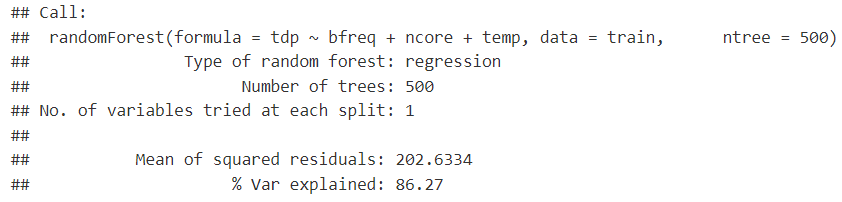
\includegraphics[width = 0.9\textwidth]{graphics/randomSum.png}
    \caption{Random Forest Regression}
    \label{fig:randomForest}
\end{figure}

In the output above, the “$\%$ Var explained” (percentage of variance explained) is a measure of the amount of variation in the target variable that is explained by the random forest regression model. Specifically, it represents the percentage of the total variance in the target variable that is accounted for by the model, and \textit{a higher percentage of variance explained is considered better}, as it indicates that the model is able to explain a larger proportion of the variation in the target variable.

An $\%$ variance explained of $86.27\%$ is generally considered to be a good result for a random forest regression model, as it suggests that the model is able to explain a significant amount of the variation in the target variable.

Another method to test the fitness of this model is checking the \textbf{Mean Absolute Error} (MAE) of this model. The lower the MAE, the better this model validates our hypothesis. To check MAE, using the following commands:
\begin{code}{R}
# Create data frame for real tdp value and predicted tdp value
comtab.rfr <- test['tdp']
comtab.rfr['tdp_predicted'] <- as.data.frame(predict(model.rfr, newdata = test), row.names = NULL)
# Evaluate model performance
accuracy <- sum(1-abs(comtab.rfr$tdp_predicted - comtab.rfr$tdp) / comtab.rfr$tdp) / nrow(comtab.rfr)
MAE <- sum(abs(comtab.rfr$tdp_predicted - comtab.rfr$tdp)) / nrow(comtab.rfr)
print(paste("Accuracy:", accuracy))
print(paste("MAE:", MAE))
\end{code}

This yields the output in the console
\begin{figure}[H]
    \centering
    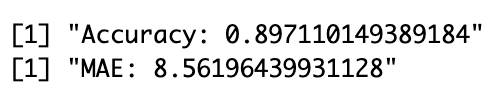
\includegraphics[width=0.45\textwidth]{graphics/MAE.png}
    \caption{Mean Absolute Error}
    \label{fig:MAE}
\end{figure}
The MAE represents the average absolute difference between the predicted and actual values of the target variable, across all observations in the data set. It is calculated by taking the mean of the absolute values of the differences between the predicted and actual values taken from the \textbf{test set} we divided before.

The acceptable level of MAE depends on the specific problem and the context in which the model is being used. In general, a lower MAE is considered better, as it indicates that the model is making more accurate predictions. In this case, the error MAE value is $8.56196$ which is relatively small compare to the range of the data, moreover, the accuracy of this model is approximately $89.711\%$, which is very high, indicating that this model is reliable. Similarly with the R-squared validation, to compute the R-squared value, we use the following commands:
\begin{code}{R}
# calculate R-squared on testing data
r2_test <- cor(comtab.rfr$tdp, comtab.rfr$tdp_predicted)^2
print(r2_test)
\end{code}

The output in the console is
\begin{figure}[H]
    \centering
    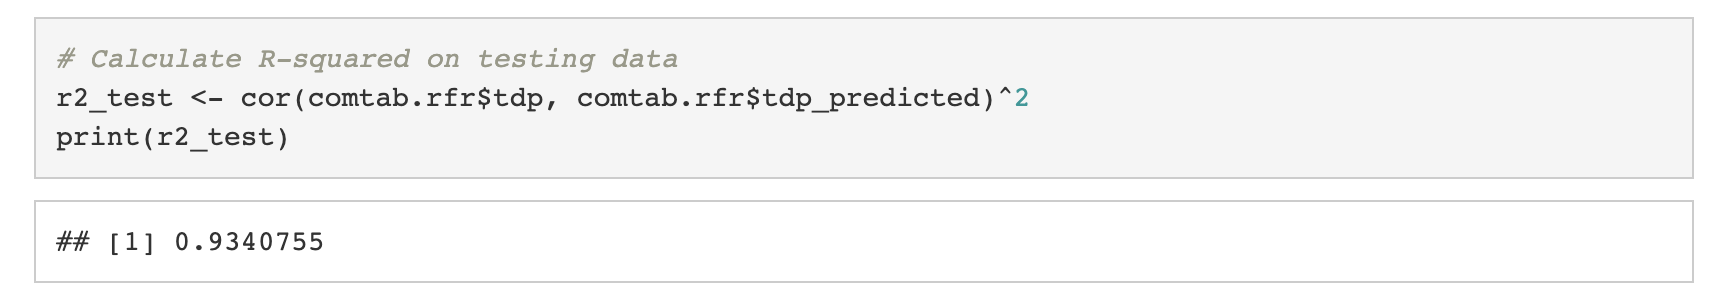
\includegraphics[width=0.9\textwidth]{graphics/RsquaredRandom.png}
    \caption{R-squared Value}
    \label{fig:RSV}
\end{figure}

Similarly in the previous model, the closer the value R-squared to 1, the more fitted the model is, which in this case is 0.9340755 very close to 1 so this strengthen the alternative hypothesis that there is a significant relationship between these features.

Because the assumption of this Random Forest model requires that the residual must follow normal distribution, we will use Q-Q plot to test if the residuals is normally distributed:
\begin{code}{R}
# Calculate the residuals by subtracting the actual values from the predicted values
residuals <- comtab.rfr$tdp - comtab.rfr$tdp_predicted

# Create a normal probability plot of the residuals
qqnorm(residuals)
qqline(residuals)
\end{code}
\begin{figure}[H]
    \centering
    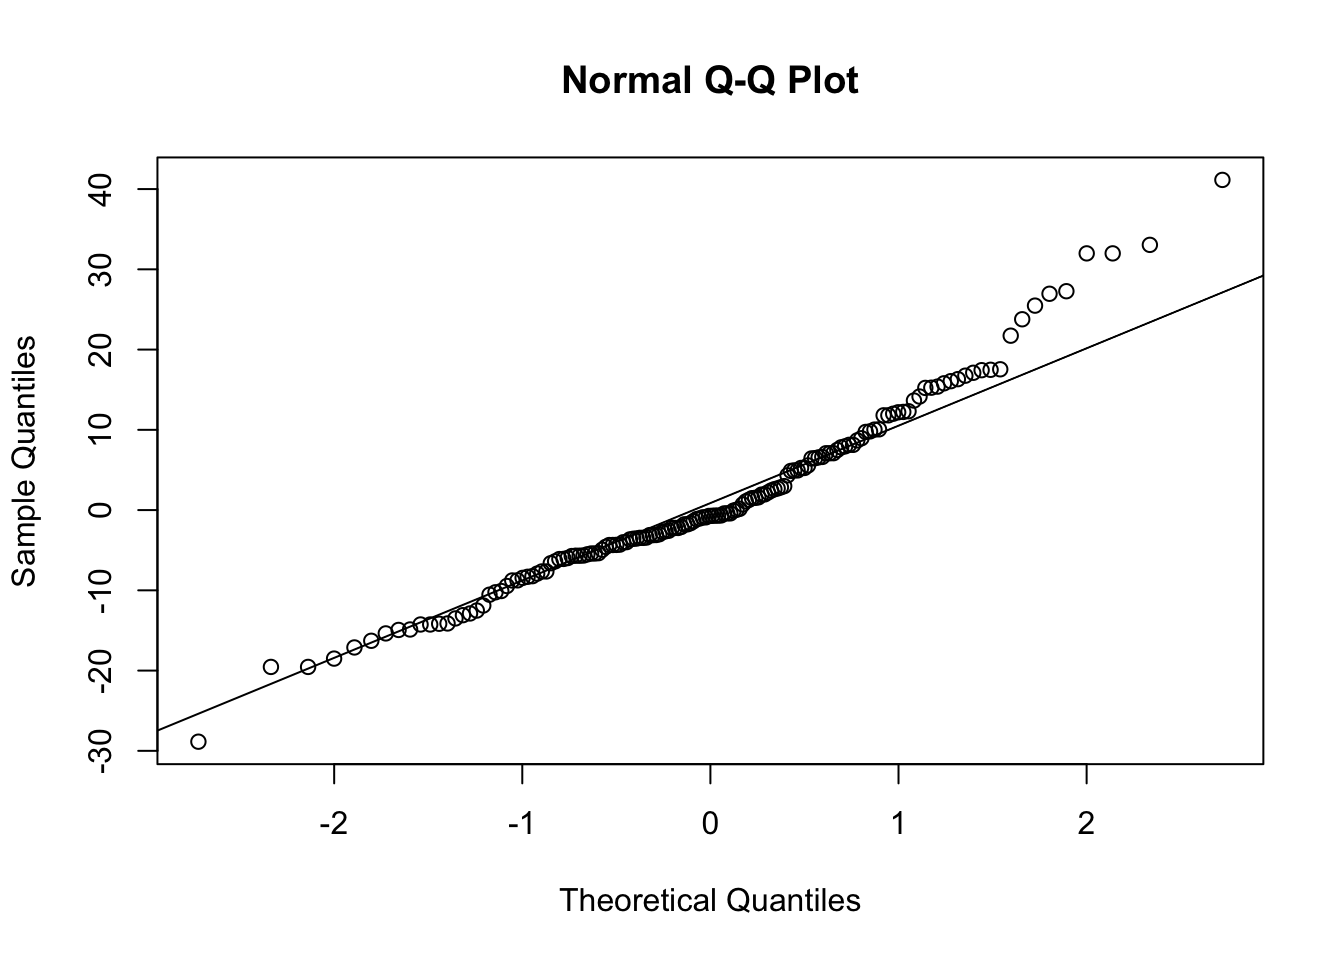
\includegraphics[width=0.9\textwidth]{graphics/randomQQplot.png}
    \caption{Theoretical quantiles Plot}
    \label{fig:QQ}
\end{figure}

In the Q-Q plot, it can be seen that those points are not fully lying near the line. We can conclude that this model may not be normally accurate.\\

We will do the scatter plotting for the predicted value of test set compared with real values of the \textbf{test} data set using \verb|plot()| function:
\begin{code}{R}
# Plot the predicted - actual
ggplot(comtab.rfr, aes(x = tdp, y = tdp_predicted)) +
  geom_point(shape = 1, color = "blue") +
  geom_abline(mapping = aes(intercept = 0, slope = 1), color = "darkblue") +
  labs(x = "TDP", y = "TDP Predicted")
\end{code}
\begin{figure}[H]
    \centering
    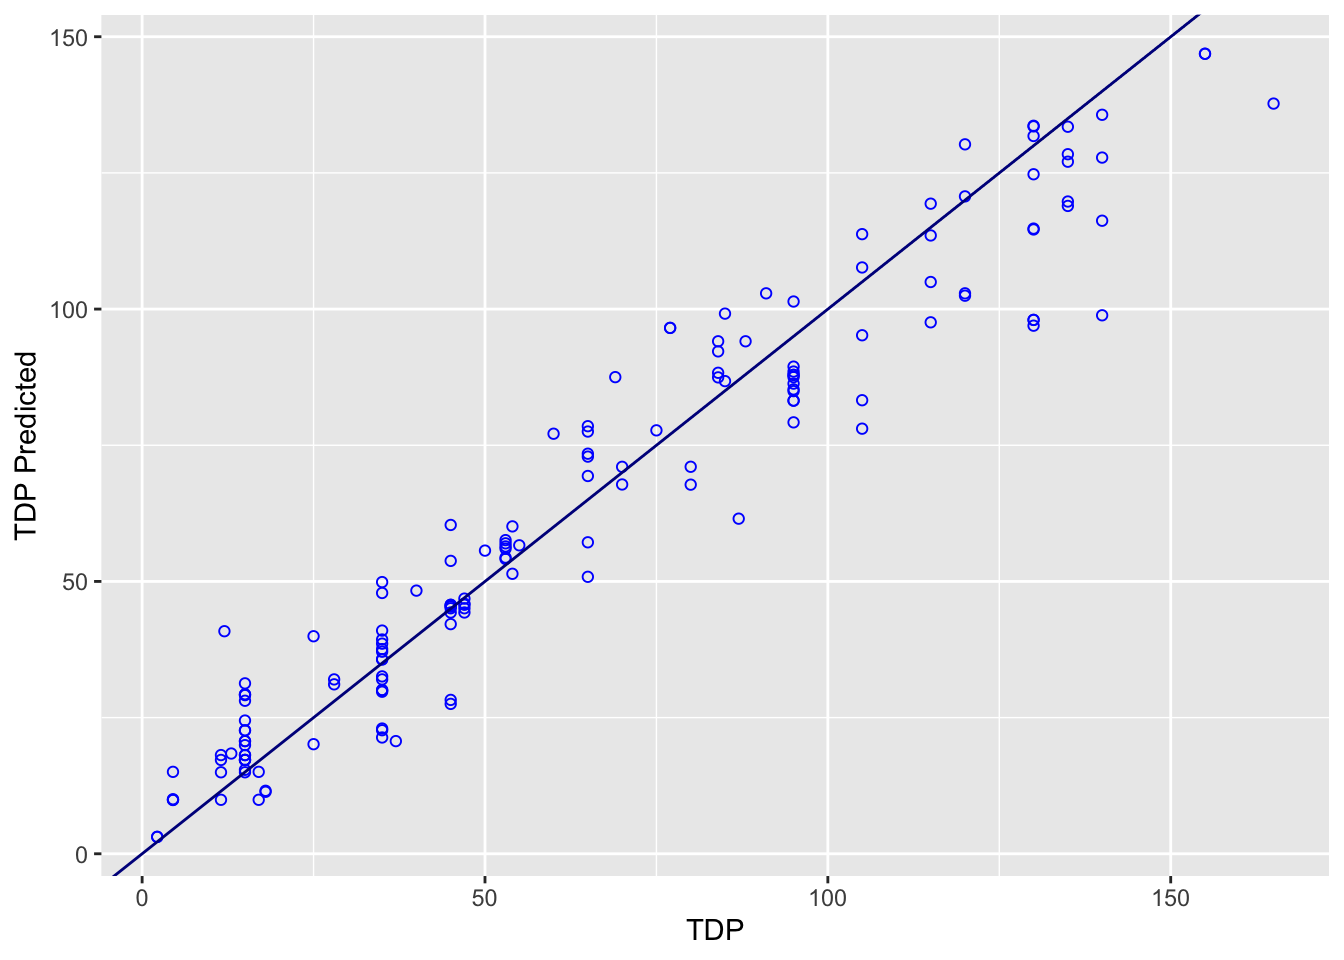
\includegraphics[width=0.7\textwidth]{graphics/randomPlot.png}
    \caption{Random Forest model prediction}
    \label{fig:random_trend}
\end{figure}

As we can see, the closer the points to the line, the more accurate the prediction, and we clearly see, similarly to the previous model, this is somewhat like $80\%$ normally distributed in residuals, which is explained most of the variables involved.

\textbf{In conclusion}, compared to Linear regression model, the current model - Random forest give us the more optimistic results which are proven in the above figures such as error, accuracy and \(R^2\) value. As a result, we conclude this model is fitter to our data and get the quite high results, not 100\% accuracy. Perhaps, more data should be obtained or some indexes such as number of tree be modified to reach the higher accuracy.













